\section{\review{Dodecapolar RDT}}

% Fill 9339
% https://logbook.cern.ch/elogbook-server#/logbook?logbookId=1081&dateFrom=2024-03-10T00%3A00%3A00&dateTo=2024-03-11T00%3A00%3A00
% http://localhost:8888/lab/workspaces/auto-Z/tree/work_afs2/jupyter/resonance_driving_terms/simulations/first_dodecapole_rdt/Plots.ipynb

During the commissioning of 2024, resonance driving terms measurements were performed by kicking the
beam at various strengths with the AC-Dipole at injection energy. Those measurements were intended
to measure several RDTs with a focus on decapoles.
However, a clear line in the vertical spectrum was observed at $5Q_y$, as shows
\cref{fig:high_orders:spectrum_dodecapole_5qy}. This line is contributed to by dodecapolar fields
(see \cref{appendix:rdts}) and is proportional to the vertical oscillation amplitude.

\begin{figure}[!htb]
    \centering
    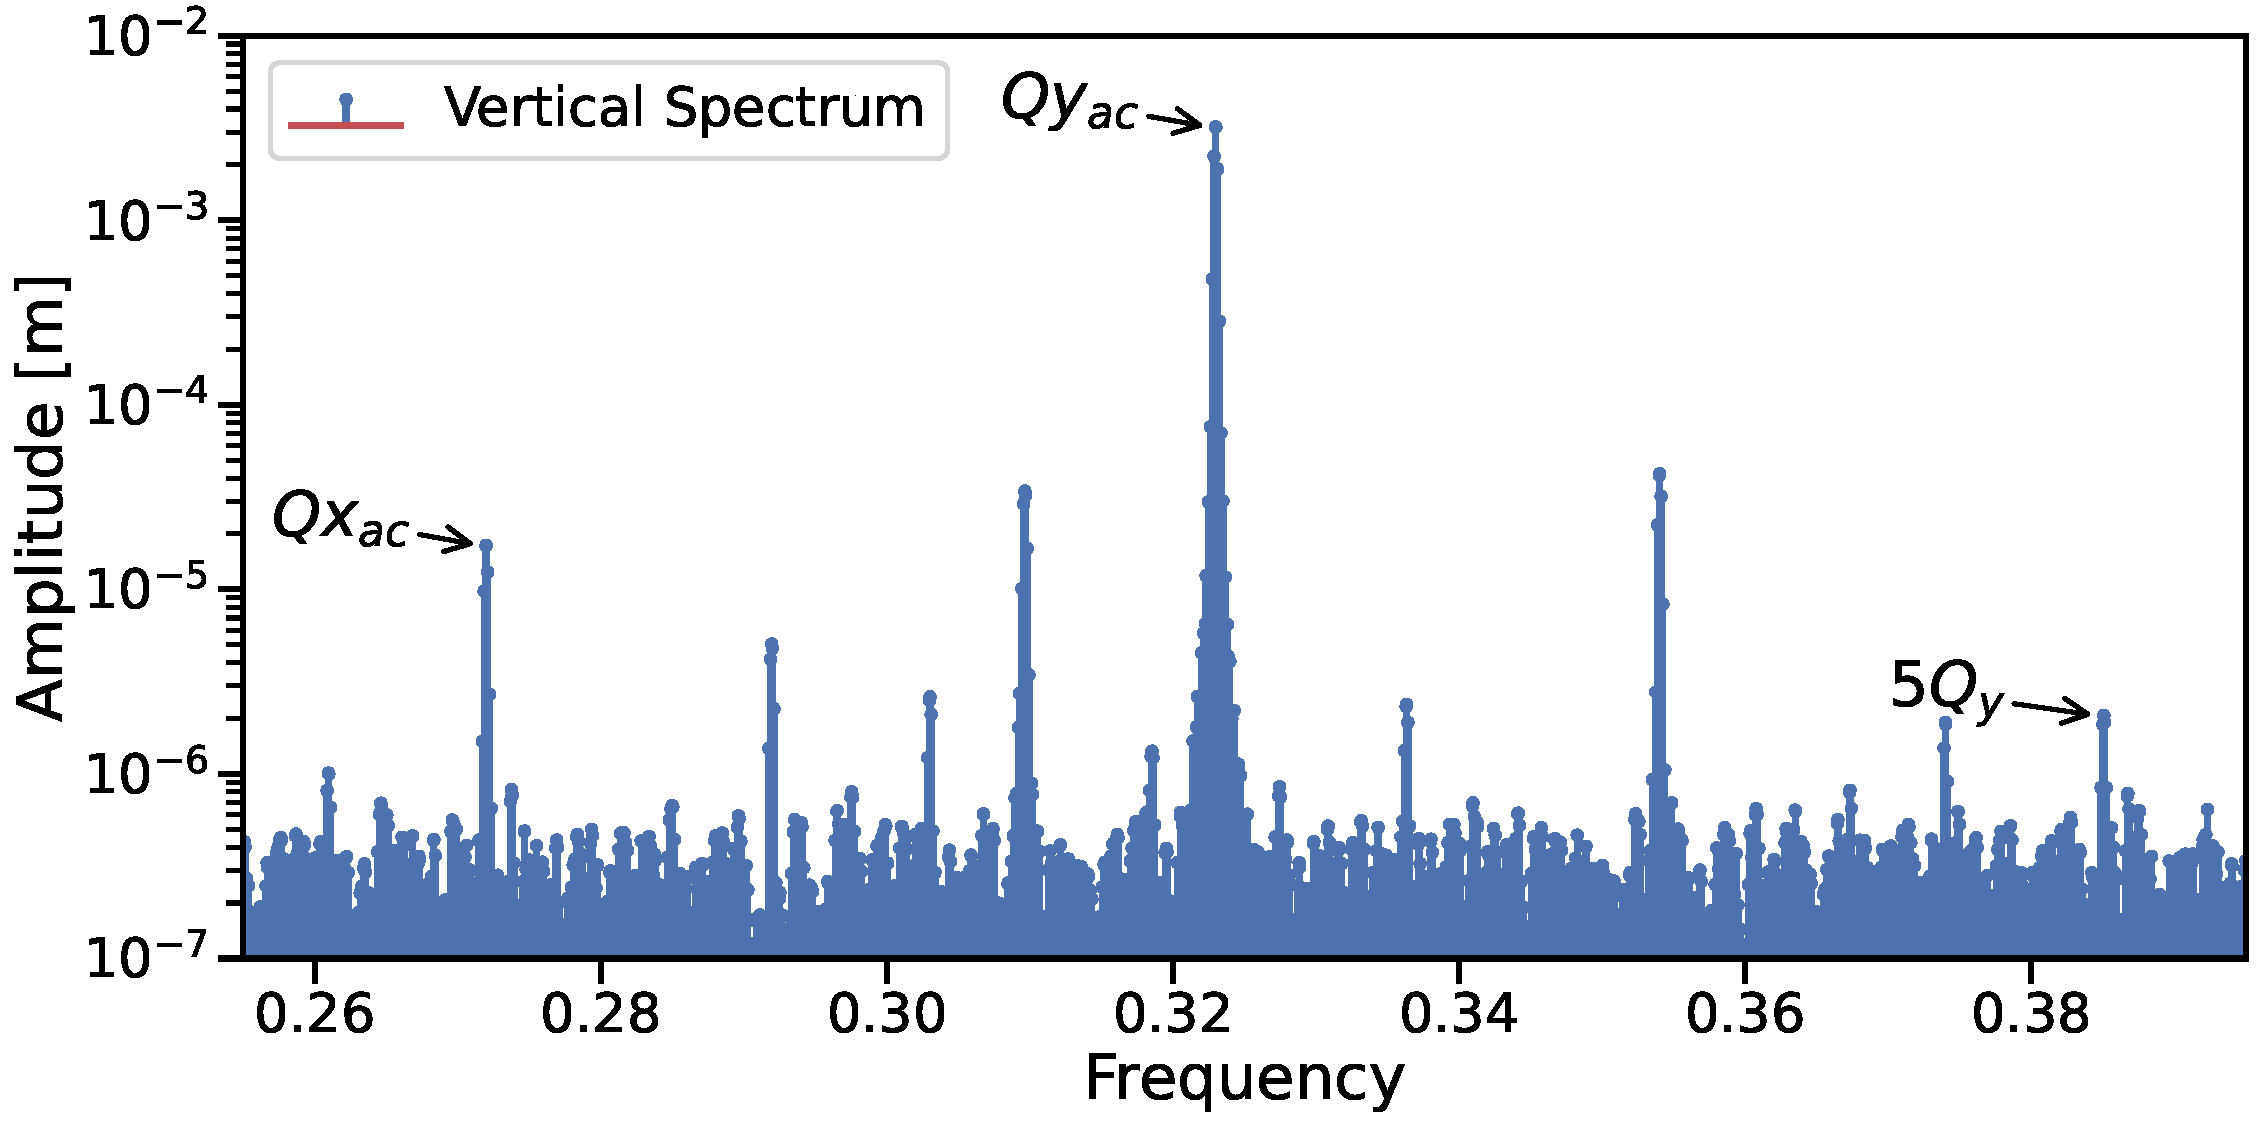
\includegraphics[width=0.8\textwidth]{./images/spectrum_dodecapole_5qy.pdf}
    \caption{Vertical spectrum of recorded turn-by-turn data for Beam 1 showing the tunes driven by the
    AC-Dipole along with a line contributed to by dodecapolar fields.}
    \label{fig:high_orders:spectrum_dodecapole_5qy}
\end{figure}

To achieve these measurements, the kick strength of the AC-Dipole was set up to $40\%$ of its
maximum, made possible by the newly introduced collimator sequence. The specific excited resonance
of the observed line is the $6Q_y$, related to the RDT $f_{0060}$.
\Cref{fig:high_orders:dodecapolar_f0060} highlights the real part of this RDT and the repeatability
of the measurement at varying kick strengths. The RMS amplitude of the average of those measurements
is of $3.5\cdot10^8$

\begin{figure}[!htb]
    \centering
    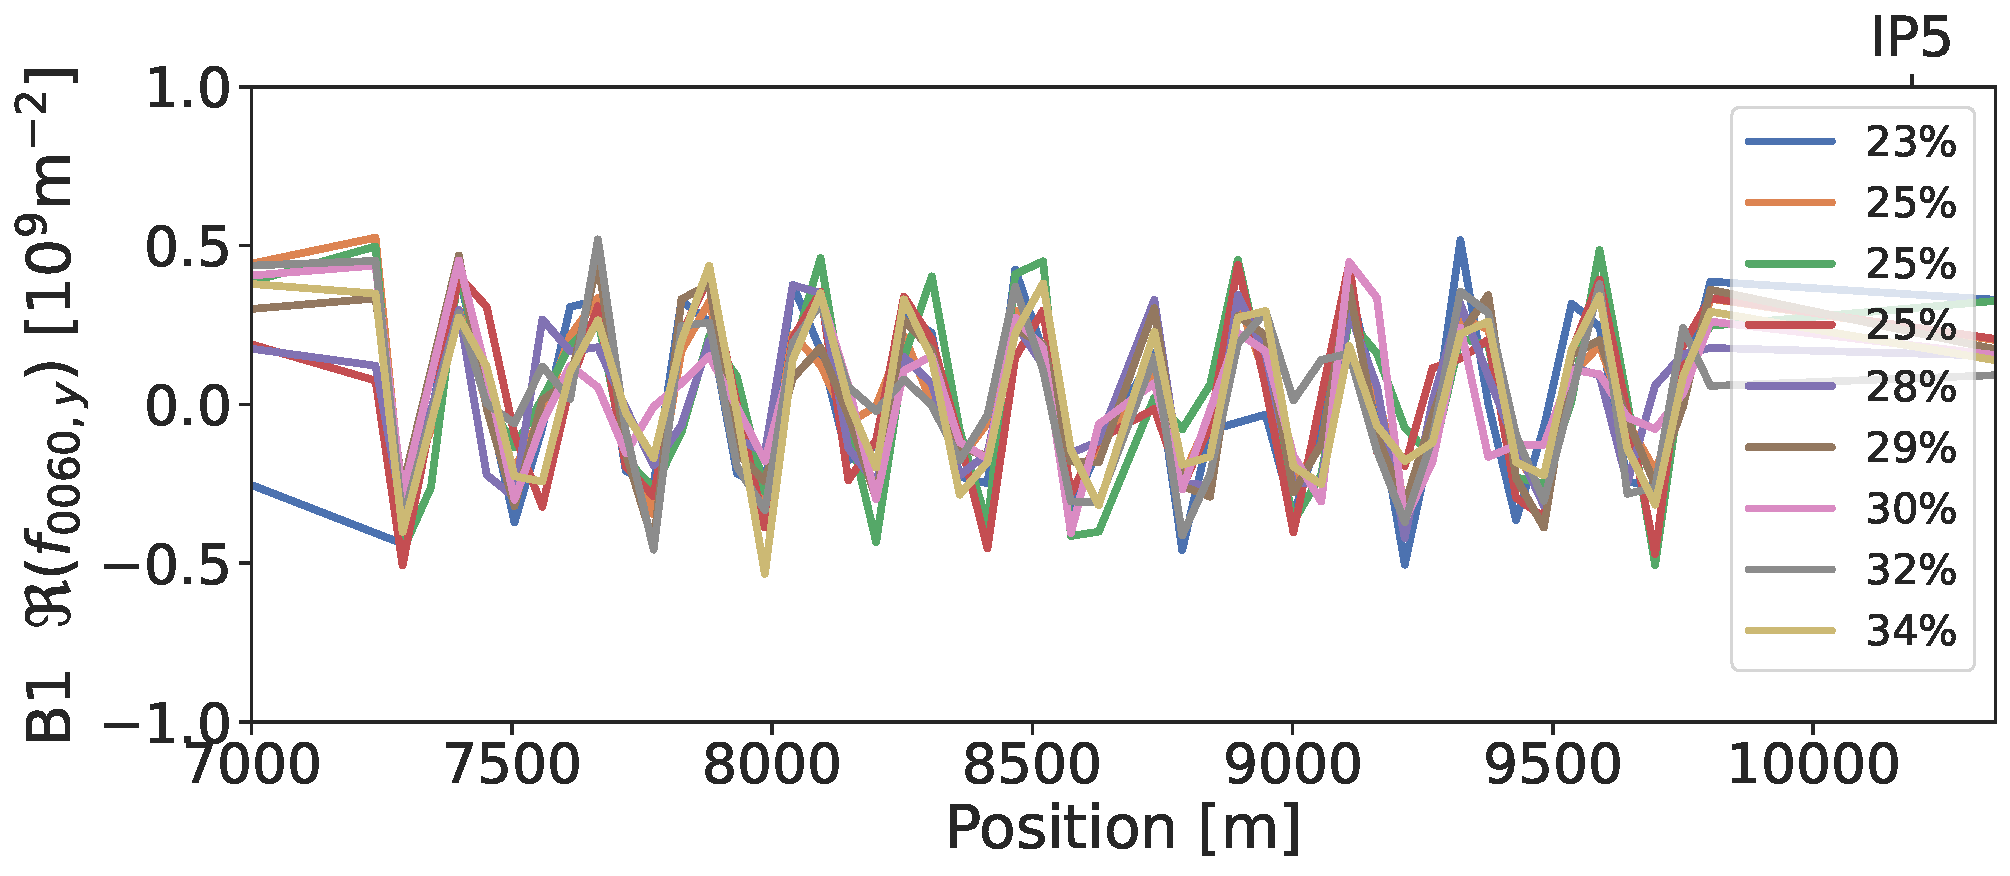
\includegraphics[width=0.8\textwidth]{./images/f0060y_all_meas_real.pdf}
    \caption{Real part of the dodecapolar RDT $f_{0060}$ measured with several kick strengths. The
    RMS amplitude is of $3.5\cdot10^{8}$.}
    \label{fig:high_orders:dodecapolar_f0060}
\end{figure}

Similar to the decapoles discussed in \cref{section:decapoles:feed_up}, the dodecapolar RDTs can be
influenced by lower-order components, as shown in
\cref{table:appendix:transfer_maps:bch_resulting_orders_combination}. At the second-order BCH, a
combination of sextupoles and decapoles, as well as a combination of octupoles, generate a
decapolar-like field. At the third and fourth orders, these fields are respectively generated by a
combination of sextupoles with octupoles and by sextupoles.

Several tracking simulations were run with various combinations of field errors, ranging from normal
and skew sextupoles ($a,b_3$) to decaoctupoles ($a,b_9$), including as well coupling, and
beta-beating via $b_2$ errors. \Cref{fig:high_orders:simulations_f0060} shows the RMS amplitude of
the RDT $f_{0060}$ resulting from those simulations. As expected from the analytical equations, the
lower-order multipoles do contribute to this RDT. The previously shown measurement is also compared
to the simulations. The contributions of the various field error combinations seem to cancel each
other and the measurement to be closed to our model. However, it is important to note that
predicting the contributions from lower-order multipoles remains difficult.

\begin{figure}[!htb]
    \centering
    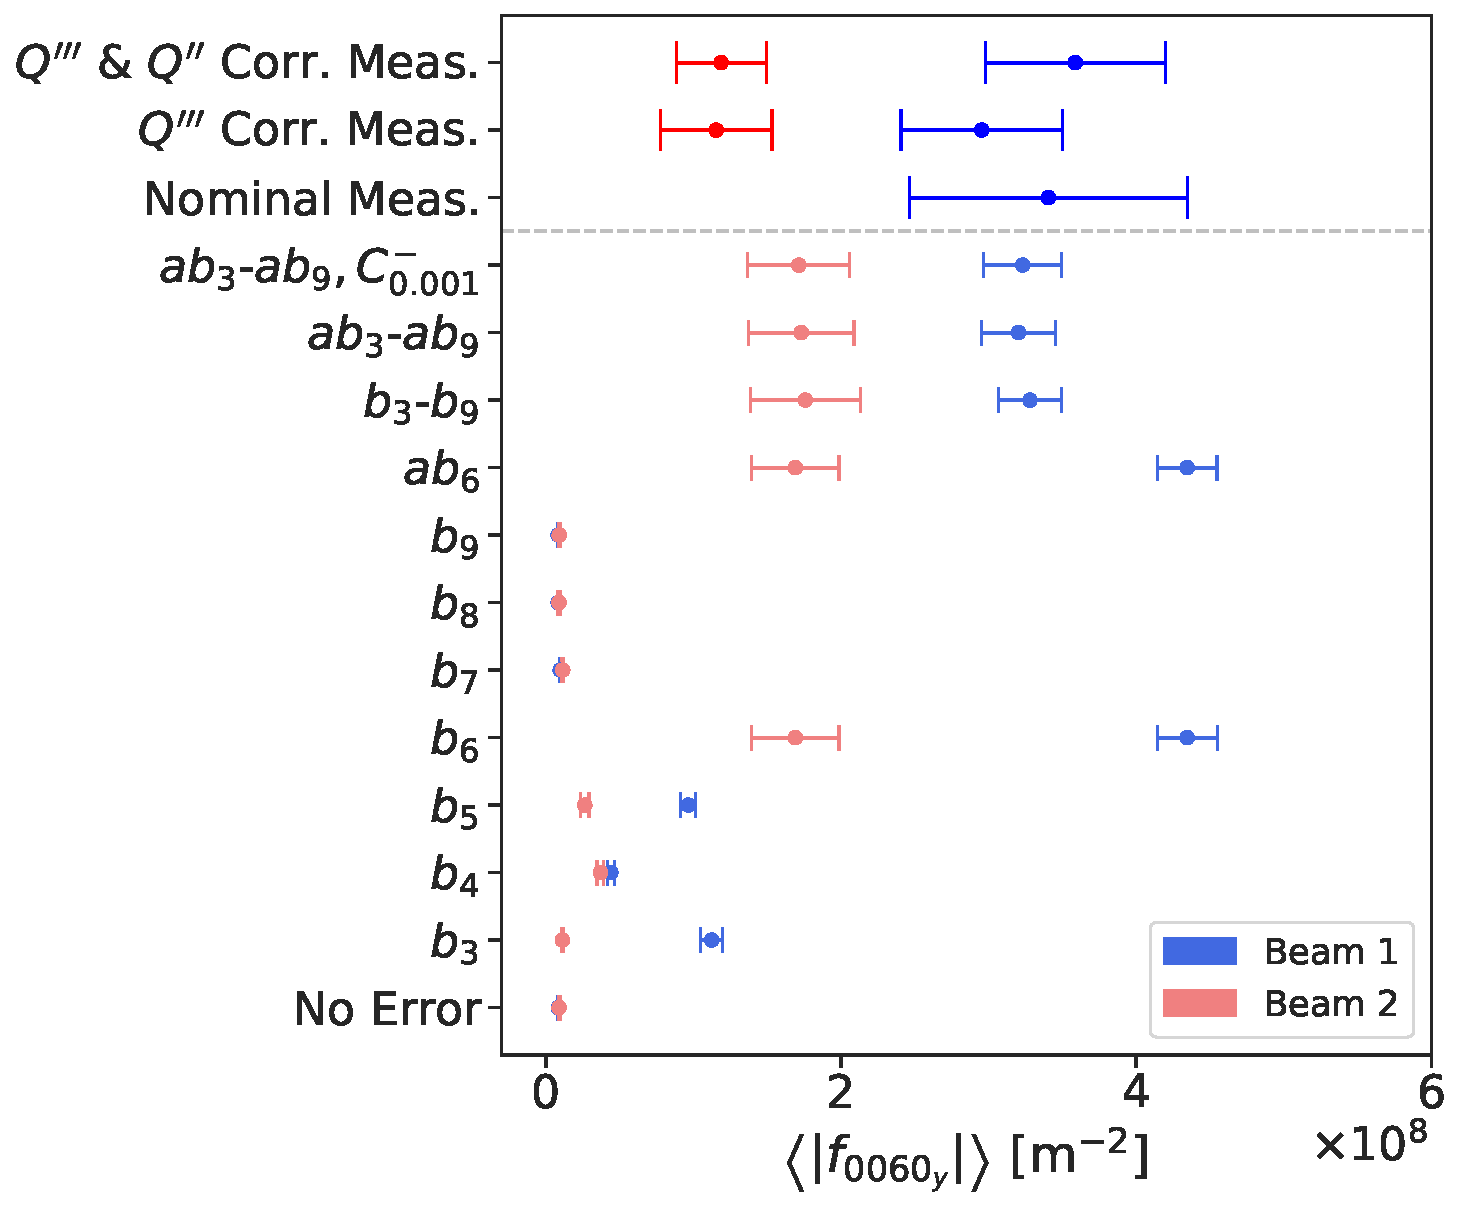
\includegraphics[width=0.8\textwidth]{./images/simulations_f0060.pdf}
    \caption{}
    \label{fig:high_orders:simulations_f0060}
\end{figure}
